
\section{Background}
\label{sec:background}

In this section, we review the dragonfly topology, including the placement and routing policies examined in previous work. 

\subsection{Dragonfly Network}
\label{sec:network}
The dragonfly is a two-level hierarchical topology, consisting of several groups connected by all-to-all links. In each group, there could be $a$ routers connected via all-to-all local channels. For each router, there could be $p$ compute nodes attached to it via terminal links. The router has $h$ global channels used as intergroup connections through which the router connected to other routers in different groups. Thus, the radix of each router is $k = a+h+p-1$. Different computing centers could choose different values for  $a$, $h$, $p$ when deploying their dragonfly network. The adoption of proper $a$, $h$, $p$ involves many factors, such as system scale, building cost and workload. 

It is recommended that for the load balance purpose, a proper dragonfly configuration should follow $a=2p=2h$~\cite{kim-micro}. Under this configuration, the total number of groups, denoted as $g$ in the dragonfly network would be $g = a*h+1 $, the total number of compute nodes denoted as $N$ in the network would be $N = p*a*g $. An implementation of dragonfly network follows such configuration is illustrated in Figure~\ref{fig:dragonfly-overview}. There are six routers in each group, each router has three compute nodes attached to it. This dragonfly network consists of 19 groups and 342 nodes in total.

\begin{figure}[h!] 
  \centering
  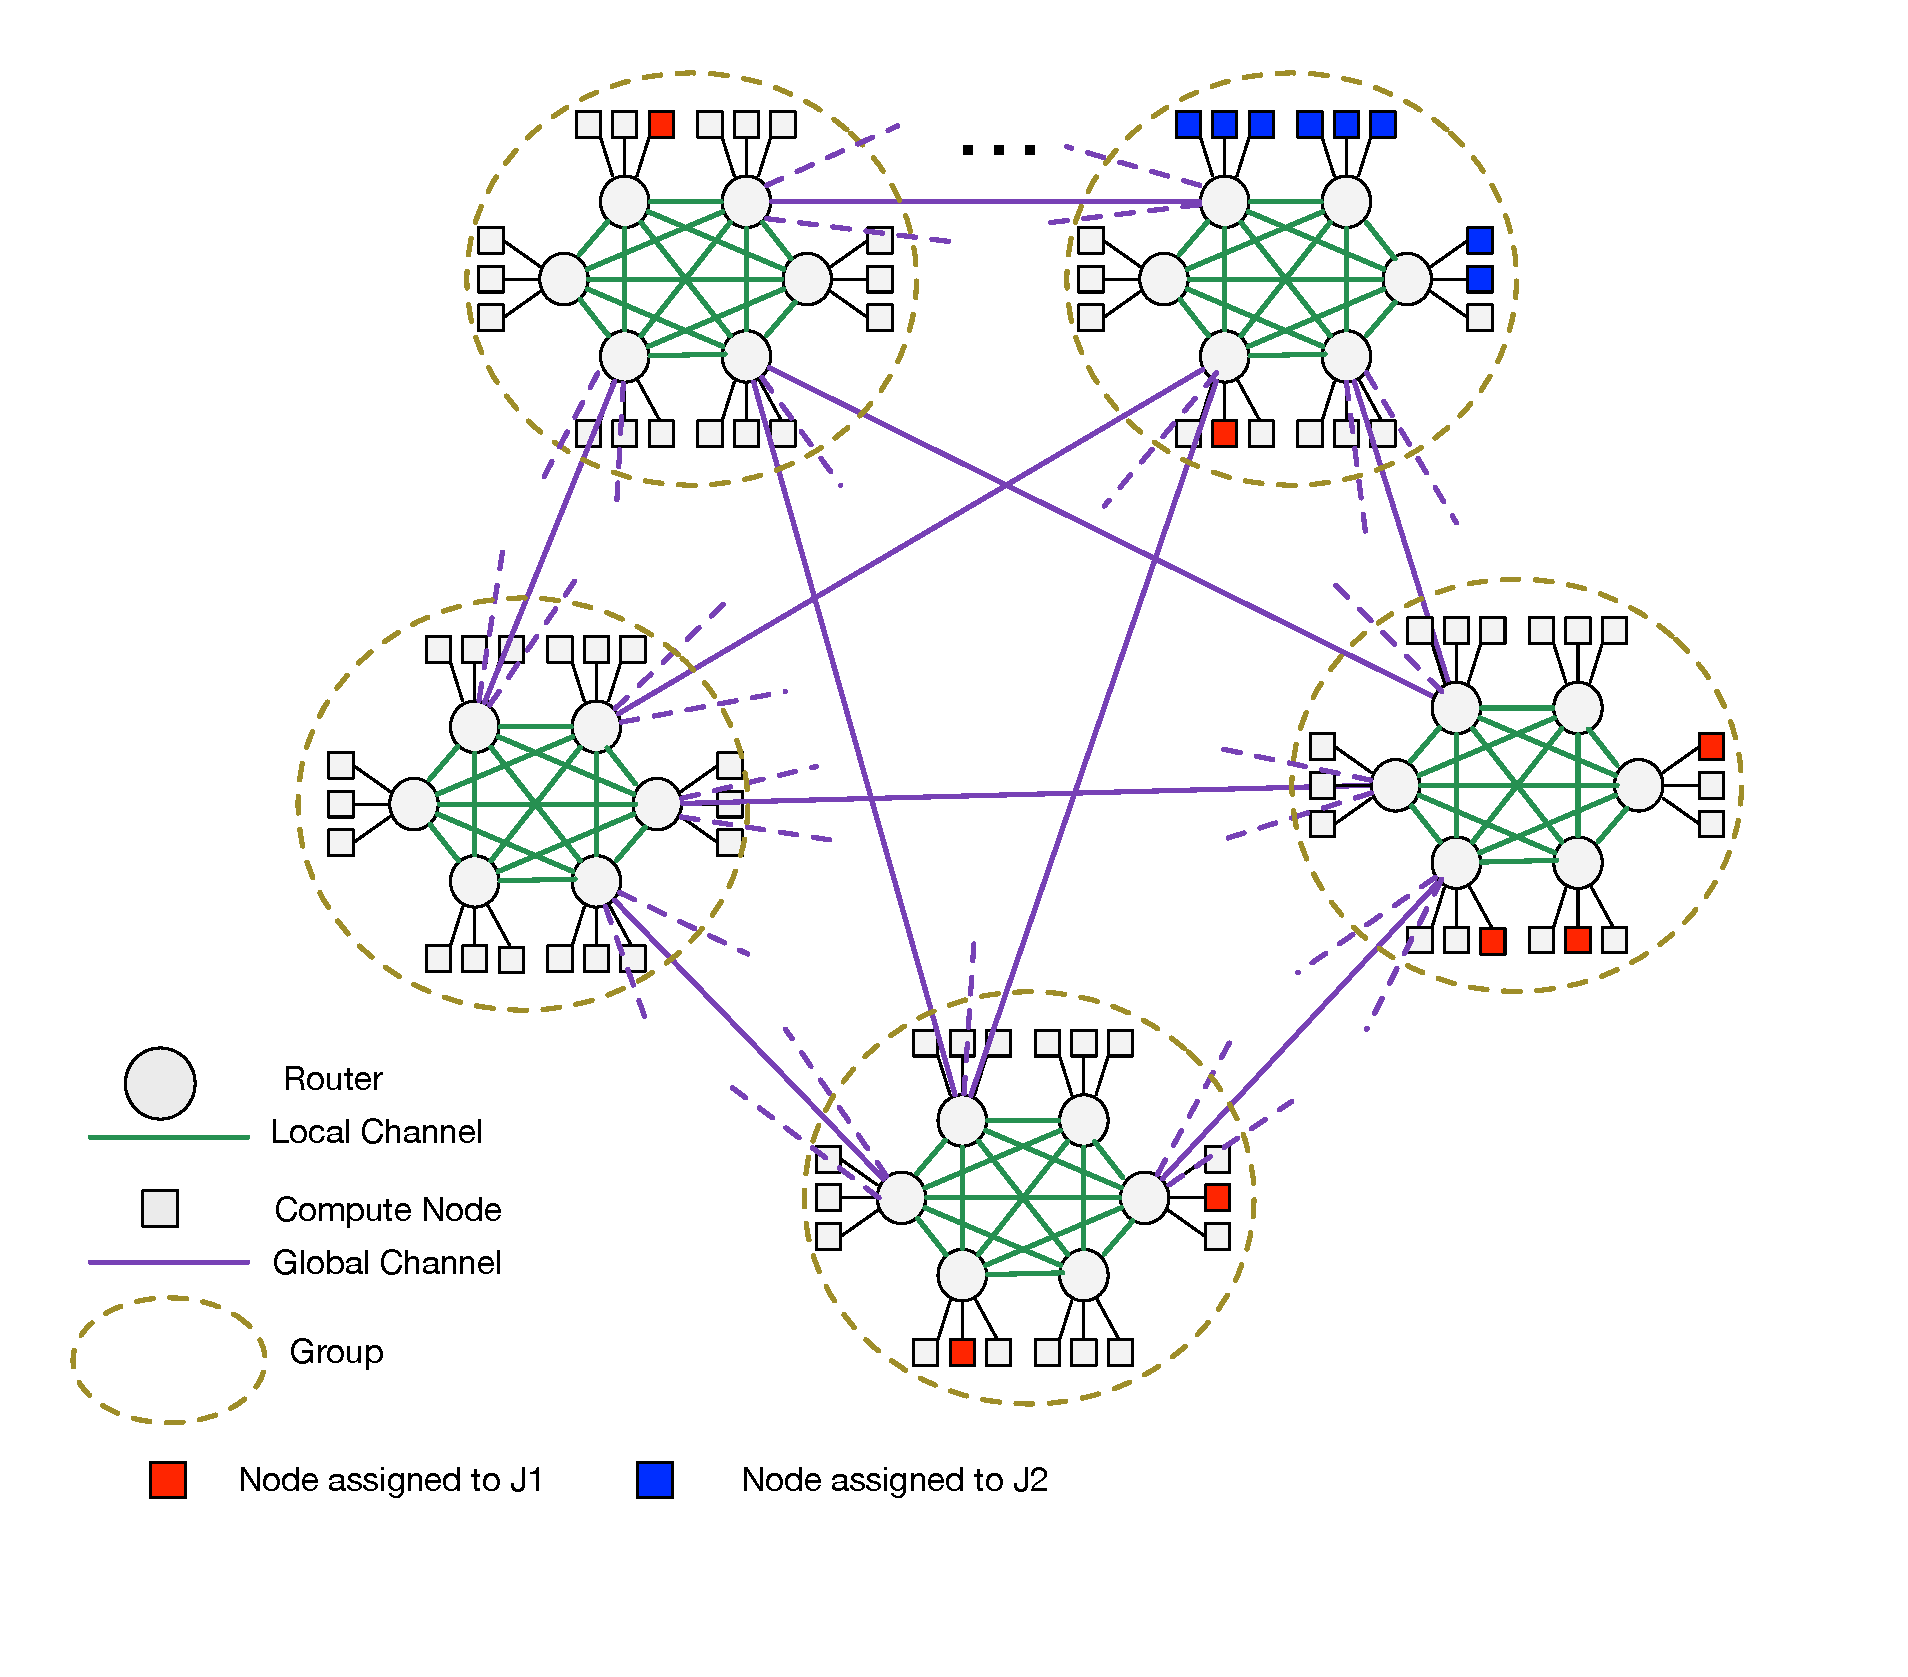
\includegraphics[width=0.48\textwidth]{dragonfly-overview}
  \caption{Dragonfly Network Overview. There are 19 groups, six routers in each group, three compute nodes connected to each router, 342 nodes in total. Job $J1$ requires seven nodes, getting its allocation by random placement. Job $J2$ requires eight nodes, getting its allocation by contiguous placement.}
  \label{fig:dragonfly-overview}
\end{figure}


\subsection{Job Placement on Dragonfly}
\label{sec:placement-schemes}

For a parallel application requiring multiple compute nodes, job placement policy refers to the way of assigning tasks of the application onto the system by a system software such as batch scheduler~\cite{xu-cluster14}. In this work, we study two alternative placement policies considered by the community for dragonfly systems: 


\textbf{Contiguous Placement:} In this policy, the compute nodes are assigned to a job in a consecutive manner. The assignment first fills up a group, then crosses group boundaries and starts to fill the next group if necessary. As shown in Figure~\ref{fig:dragonfly-overview}, $J2$ gets eight nodes by contiguous placement. Contiguous placement confines the tasks of a job into the same group, which may result in local network congestion and increase the possibility of hot-spots. 

\textbf{Random Placement:} In this policy, a job gets a set of nodes randomly selected from all the available nodes in the system. The nodes assigned to $J1$ in Figure~\ref{fig:dragonfly-overview} are attached to different routers in different groups. Routers may be shared by different jobs when random placement is in use. Random placement can distribute the tasks of a job uniformly across the whole system to avoid the possible local congestion. However, random placement may cause possible congestion on global links.


\subsection{Routing on Dragonfly}
\label{sec:routing-schemes}

The routing policy refers to the strategy adopted to route a message (a stream of packets) from the source router to the destination router. Previously studied routing policies for dragonfly network include minimal routing, adaptive routing~\cite{dally-dragonfly}, progressive adaptive routing~\cite{jiang} and some of their variations~\cite{won-prog-adaptive}. In this work we study three widely adopted routing policies on dragonfly networks.

\textbf{Minimal:} In this policy, a message takes the shortest path from the source router to the destination router. When there are multiple shortest paths between the source and destination router, the message will be evenly divided among the paths. Minimal routing can guarantee the minimum hops the message takes from source to destination. However, it may result in congestion along the shortest path. 

\textbf{Adaptive:} In this policy, the path a message takes will be adaptively chosen between shortest and non-shortest paths, depending on the congestion situation along those paths. For the non-shortest path, an intermediate router will be randomly chosen. The message takes the intermediate router as a via point, connecting the source and destination router through two separate shortest paths. Adaptive routing can avoid hot-spots in the presence of congestion and collapse to minimal routing otherwise. 

\textbf{Progressive Adaptive:} In this policy, the decision to route minimally at each hop in the source group will be re-evaluated. Any decision to route non-minimally at source router or at a subsequent hop is permanent and will not be re-evaluated~\cite{jiang}. The progressive adaptive is capable of handling the case where a global channel is congested but the source router has not been informed yet~\cite{jiang}. The packet will take the non-minimal route only when the congestion is encountered. 


